% Jacob Neumann

% DOCUMENT CLASS AND PACKAGE USE
    \documentclass[aspectratio=169]{beamer}
 
    % Establish the colorlambda boolean, to control whether the lambda is solid color (true), or the same as the picture (false)
    \newif\ifcolorlambda
    \colorlambdafalse % DEFAULT: false
    
    % Use auxcolor for syntax highlighting
    \newif\ifuseaux
    \useauxfalse % DEFAULT: false
   
    % Color settings
    \useauxtrue
    
    \newcommand{\auxColor}{6e3b0d}     % the color of note boxes and stuff
    \newcommand{\presentColor}{FFABE1} % the primary color of the slide borders
    \newcommand{\bgColor}{fef7ff}      % the color of the background of the slide
    \newcommand{\darkBg}{8b98ad}
    \newcommand{\lambdaColor}{\auxColor}
  
    \colorlambdatrue

    \usepackage{comment} % comment blocks
    \usepackage{soul} % strikethrough
    \usepackage{listings} % code
    \usepackage{makecell}

    \setbeamertemplate{itemize items}[circle]
    % \setbeameroption{show notes on second screen=right}

    \usepackage{lectureSlides}
    %%%%%%%%%%%%%%%%%%%%%%%%%%%%%%%%%%%%%%%%%| <----- Don't make the title any longer than this
    \title{Trees} % TODO
    \subtitle{Branching out our types} % TODO
    \date{30 May 2023} % TODO
    \author{Brandon Wu} % TODO

    \graphicspath{ {./img/} }
    % DONT FORGET TO PUT [fragile] on frames with codeblocks, specs, etc.
        %\begin{frame}[fragile]
        %\begin{codeblock}
        %fun fact 0 = 1
        %  | fact n = n * fact(n-1)
        %\end{codeblock}
        %\end{frame}

    % INCLUDING codefile:
        % 1. In some file under code/NN (where NN is the lecture id num), include:
    %       (* FRAGMENT KK *)
    %           <CONTENT>
    %       (* END KK *)
    
    %    Remember to not put anything on the same line as the FRAGMENT or END comment, as that won't be included. KK here is some (not-zero-padded) integer. Note that you MUST have fragments 0,1,...,KK-1 defined in this manner in order for fragment KK to be properly extracted.
        %  2. On the slide where you want code fragment K
                % \smlFrag[color]{KK}
        %     where 'color' is some color string (defaults to 'white'. Don't use presentColor.
    %  3. If you want to offset the line numbers (e.g. have them start at line 5 instead of 1), use
                % \smlFragOffset[color]{KK}{5}

\begin{document}

% Make it so ./mkWeb works correctly
\ifweb
    \renewcommand{\pause}{}
\fi

\setbeamertemplate{itemize items}[circle]

% SOLID COLOR TITLE (see SETTINGS.sty)
{
\begin{frame}[plain]
    \colorlambdatrue
    \titlepage
\end{frame}
}

\begin{frame}[fragile]
  \frametitle{Last time}

  Last time, we learned about the technique of \term{structural induction} for lists, and
  used it to prove some theorems about functions on lists.

  \vspace{\fill}

  We also learned about \term{tail recursion}, and how it can help make code more efficient. We
  used \term{accumulators} to facilitate the implementation. We also implemented some useful
  functions on lists.
\end{frame}

\begin{frame}[fragile]
  \frametitle{Lesson Plan}

  \tableofcontents
\end{frame}

\sectionSlide{1}{Trees}

\begin{frame}[fragile]
  \frametitle{Data Structures}

  In computer science, there are only a few fundamental data structures, from which everything
  else pretty much is derived from.

  \pause
  \vspace{\fill}

  One of them is lists, which we've already covered. The other is \term{trees}.

  \pause
  \vspace{\fill}

  \defBox{}{\, A \term{binary tree} is a data structure of nodes, where each node may have up
  to two children that are also binary trees.}

  \pause
  \vspace{\fill}

  They look something like this:

  \vspace{\fill}

  \begin{center}
    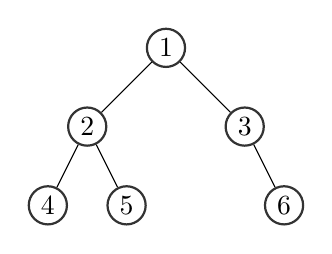
\begin{tikzpicture}
      [level distance=10mm,
      every node/.style={circle,inner sep=2pt, draw=black!80, thick},
      level 1/.style={sibling distance=20mm},
      level 2/.style={sibling distance=10mm},
      ]
      \node {1}
        child {node {2}
          child {node {4}}
          child {node {5}}
        }
        child {node {3}
          child[missing] 
          child {node {6}}
        };
      \end{tikzpicture}
  \end{center}
\end{frame}

\begin{frame}[fragile]
  \frametitle{Trees}

  SML doesn't have an in-built notion of trees, the same way that it does lists, but we can
  define our own. We can use a \term{datatype declaration} to achieve this.

  \pause
  \vspace{\fill}

  \defBox{}{\, A \term{datatype declaration} is a declaration in SML, which declares a new
  type.}

  \pause
  \vspace{\fill}

  A datatype declaration for binary trees on integers would look something like this:
  \begin{codeblock}
    datatype tree = Empty | Node of tree * int * tree
  \end{codeblock}
\end{frame}

\begin{frame}[fragile]
  \frametitle{Tree Constructors}

  \begin{codeblock}
    datatype tree = Empty | Node of tree * int * tree
  \end{codeblock}
  
  \vspace{\fill}

  This datatype declaration does two things. Firstly, it declares a new type, named \code{tree}.
  Secondly, it provides that type with two \term{constructors}, in the same way as the constructors 
  that we saw earlier for lists.

  \pause
  \vspace{\fill}

  This declaration says that:
  \pause
  \begin{itemize}
    \item \code{Empty : tree} \pause
    \item \code{Node (L, x, R) : tree} if and only if \code{L : tree}, \code{x : int}, and \code{R : tree}. \pause
  \end{itemize}

  \vspace{\fill}

  In essence, it's saying that a tree only takes two forms, \code{Empty} or \code{Node (L, x, R)}. A tree
  is one of those two things, and \textbf{no more}.
\end{frame}

\begin{frame}[fragile]
  \frametitle{Tree Examples}

  Let's see some examples of trees, and how they would be pictured visually\footnotemark:

  \pause
  \vspace{\fill}

  \code{Empty : tree}

  \begin{center}
    (nothing pictured)
  \end{center}

  \pause
  \vspace{\fill}

  \code{Node(Empty, 150, Empty) : tree}

  \begin{center}
    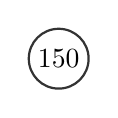
\begin{tikzpicture}
      [level distance=10mm,
      every node/.style={circle,inner sep=2pt, draw=black!80, thick},
      level 1/.style={sibling distance=20mm},
      level 2/.style={sibling distance=10mm},
      ]
      \node {150}
        child[missing] 
        child[missing];
      \end{tikzpicture}
  \end{center}

  \footnotetext[1]{It can be confusing to type out a tree in text, so 
  if you need help, you can refer to {\color{blue}\href{https://leesue630.github.io/tree-to-sml-converter/}{this excellent
  SML tree converter}}, which lets you generate SML text for trees from pictures and
  pictures from SML text, made by previous head TA Sue Lee.}
\end{frame}

\begin{frame}[fragile]
  \frametitle{Tree Examples}

  \code{Node(Node(Empty, 1, Empty), 5, Node(Empty, 0, Empty)) : tree}

  \begin{center}
    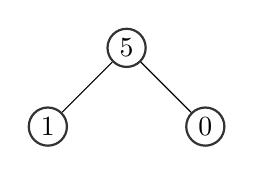
\begin{tikzpicture}
      [level distance=10mm,
      every node/.style={circle,inner sep=2pt, draw=black!80, thick},
      level 1/.style={sibling distance=20mm},
      level 2/.style={sibling distance=10mm},
      ]
      \node {5}
        child {node {1}}
        child {node {0}};
      \end{tikzpicture}
  \end{center}

  \pause
  \vspace{\fill}

  \code{Node(Node(Empty, 1, Empty), 5, Empty) : tree}

  \begin{center}
    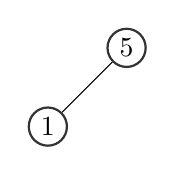
\begin{tikzpicture}
      [level distance=10mm,
      every node/.style={circle,inner sep=2pt, draw=black!80, thick},
      level 1/.style={sibling distance=20mm},
      level 2/.style={sibling distance=10mm},
      ]
      \node {5}
        child {node {1}}
        child [missing];
      \end{tikzpicture}
  \end{center}
\end{frame}

\begin{frame}[fragile]
  \frametitle{Constructors}

  \rprs

  The syntax is important to get used to.

  \pause
  \vspace{\fill}

  Of our two constructors for the \code{tree} datatype, only one takes an argument. The other is
  \code{Empty}, which is called a \term{constant constructor}. It requires no arguments in order
  to be a value of type \code{tree}.

  \pause
  \vspace{\fill}

  The constructor that takes an argument is \code{Node}, which takes in a tuple of type
  \code{tree * int * tree}. This type uses the \code{tree} type we are in the middle of defining!

  \pause
  \vspace{\fill}

  This is allowed, and called a \term{recursive type}. Datatypes are allowed to be recursive,
  in essence saying that the \code{tree} type can be built out of other \code{tree}s, with the
  \code{Node} constructor.
\end{frame}

\begin{frame}[fragile]
  \frametitle{Tree Functions}

  We can write functions on trees using pattern matching, in the same way that we
  write functions on lists.

  \pause
  \vspace{\fill}

  For instance, let's write a function which sums all the nodes of a tree:

  \begin{codeblock}
    fun treesum (Empty : tree) : int = 0
      | treesum (Node (L, x, R)) = treesum L + x + treesum R
  \end{codeblock}

  \pause
  \vspace{\fill}

  When writing recursive functions on trees, we need two recursive calls instead of one
  for lists!
\end{frame}

\begin{frame}[fragile]
  \frametitle{Getting In-\code{depth}}

  Let's write a simple function for computing the depth of a tree.

  \pause
  \begin{codeblock}
    fun max (x : int, y : int) : int =
      if x < y then x else y

    fun depth (Empty : tree) : int = 0
      | depth (Node (L, x, R)) = 1 + max (depth L, depth R) 
  \end{codeblock}

  \vspace{\fill}

  \customBox{Check your understanding}{\, Why was this function not written
  by just directly comparing \code{depth L} and \code{depth R}?}

  \note {
    Why did I not write it by just comparing depth L and depth R?
  }
\end{frame}

% TODO: i need to talk about totality citations
\sectionSlide{2}{Tree Traversals}

\begin{frame}[fragile]
  \frametitle{Boilerplate Tree Code}

  Sometimes, we are interested in converting data between lists and trees.

  \pause
  \vspace{\fill}

  In particular, we might be interested in quantities such as determining the
  number of nodes in a tree. We could, of course, roll our own function to do
  so:

  \pause
  \begin{codeblock}
    fun count (Empty : tree) : int = 0 
      | count (Node (L, x, R)) = count L + 1 + count R
  \end{codeblock}

  \pause
  \vspace{\fill}

  But this is kind of boilerplate code, and we might want to avoid having to
  write this!  
\end{frame}

\begin{frame}[fragile]
  \frametitle{Tree Traversals}

  We already have a function for counting the number of elements in a \textit{list},
  however.

  \pause
  \vspace{\fill}

  What if we could turn a tree into a list? We need a function of type 
  \code{tree -> int list}, which defines a kind of \term{traversal}.

  \pause
  \vspace{\fill}

  \defBox{}{\, A \term{tree traversal} is a particular kind of way to visit the
  elements in a tree. They come in three main kinds, \term{preorder}, \term{postorder},
  and \term{inorder}.}

  \pause
  \vspace{\fill}

  \begin{minipage}{0.32\textwidth}
    \begin{center}
      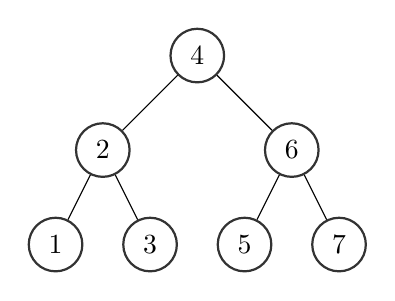
\begin{tikzpicture}
        [level distance=12mm,
        every node/.style={circle,inner sep=4pt, draw=black!80, thick},
        level 1/.style={sibling distance=24mm},
        level 2/.style={sibling distance=12mm},
        ]
        \node {4}
          child {node {2}
            child {node {1}}
            child {node {3}}
          }
          child {node {6}
            child {node {5}}
            child {node {7}}
          };
        \end{tikzpicture}

        Inorder
    \end{center}
  \end{minipage}
  \begin{minipage}{0.32\textwidth}
    \begin{center}
      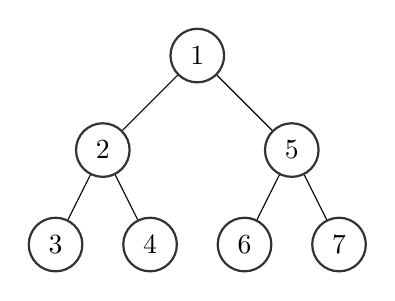
\begin{tikzpicture}
        [level distance=12mm,
        every node/.style={circle,inner sep=4pt, draw=black!80, thick},
        level 1/.style={sibling distance=24mm},
        level 2/.style={sibling distance=12mm},
        ]
        \node {1}
          child {node {2}
            child {node {3}}
            child {node {4}}
          }
          child {node {5}
            child {node {6}}
            child {node {7}}
          };
        \end{tikzpicture}

      Preorder
    \end{center}
  \end{minipage}
  \begin{minipage}{0.32\textwidth}
    \begin{center}
      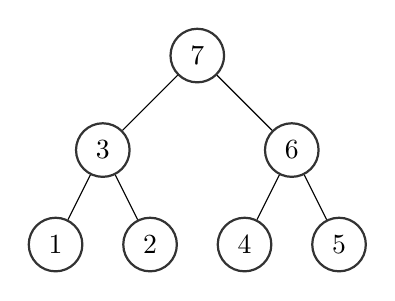
\begin{tikzpicture}
        [level distance=12mm,
        every node/.style={circle,inner sep=4pt, draw=black!80, thick},
        level 1/.style={sibling distance=24mm},
        level 2/.style={sibling distance=12mm},
        ]
        \node {7}
          child {node {3}
            child {node {1}}
            child {node {2}}
          }
          child {node {6}
            child {node {4}}
            child {node {5}}
          };
        \end{tikzpicture}

        Postorder
    \end{center}
  \end{minipage}
\end{frame}

\begin{frame}[fragile]
  \frametitle{Kinds of Traversals}
  \begin{minipage}{0.32\textwidth}
    \begin{center}
      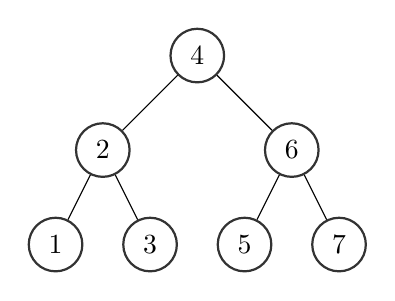
\begin{tikzpicture}
        [level distance=12mm,
        every node/.style={circle,inner sep=4pt, draw=black!80, thick},
        level 1/.style={sibling distance=24mm},
        level 2/.style={sibling distance=12mm},
        ]
        \node {4}
          child {node {2}
            child {node {1}}
            child {node {3}}
          }
          child {node {6}
            child {node {5}}
            child {node {7}}
          };
        \end{tikzpicture}
        
        \vspace{5pt}

        Inorder

        \vspace{5pt}

        {\color{black!10!red}left}-{\color{black!20!green}root}-{\color{black!10!blue}right}
    \end{center}
  \end{minipage}
  \begin{minipage}{0.32\textwidth}
    \begin{center}
      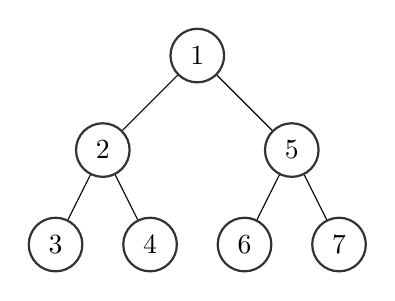
\begin{tikzpicture}
        [level distance=12mm,
        every node/.style={circle,inner sep=4pt, draw=black!80, thick},
        level 1/.style={sibling distance=24mm},
        level 2/.style={sibling distance=12mm},
        ]
        \node {1}
          child {node {2}
            child {node {3}}
            child {node {4}}
          }
          child {node {5}
            child {node {6}}
            child {node {7}}
          };
        \end{tikzpicture}

      \vspace{5pt}

      Preorder

      \vspace{5pt}

      {\color{black!20!green}root}-{\color{black!10!red}left}-{\color{black!10!blue}right}
    \end{center}
  \end{minipage}
  \begin{minipage}{0.32\textwidth}
    \begin{center}
      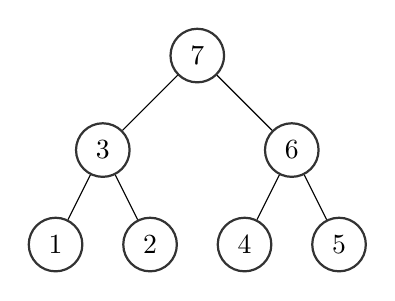
\begin{tikzpicture}
        [level distance=12mm,
        every node/.style={circle,inner sep=4pt, draw=black!80, thick},
        level 1/.style={sibling distance=24mm},
        level 2/.style={sibling distance=12mm},
        ]
        \node {7}
          child {node {3}
            child {node {1}}
            child {node {2}}
          }
          child {node {6}
            child {node {4}}
            child {node {5}}
          };
        \end{tikzpicture}

        \vspace{5pt}

        Postorder

        \vspace{5pt}

        {\color{black!10!red}left}-{\color{black!10!blue}right}-{\color{black!20!green}root}
    \end{center}
  \end{minipage}

  \vspace{\fill}

  There are three primary kinds of tree traversals, which are characterized by the
  order in which they choose to visit the left subtree, right subtree, and root. 
  We will usually be concerned with the first two kinds.

  \vspace{\fill}

  The trees are enumerated according to the order in which they are visited, in
  each traversal.
\end{frame}

\begin{frame}[fragile]
  \frametitle{Implementing Tree Traversal}

  \rprs

  Tree traversal can be implemented in SML very simply.

  \pause
  \begin{codeblock}
    fun inord (Empty : tree) : int list = []
      | inord (Node (L, x, R)) = (inord L) @ (x :: inord R)

    fun preord (Empty : tree) : int list = []
      | preord (Node (L, x, R)) = x :: ((preord L) @ (preord R))
  \end{codeblock}

  \pause
  \vspace{\fill}

  Think about how these functions are implemented, with respect to the
  recursive leap of faith! For \code{inord}, we can be assured that it
  follows the left-root-right order, because recursively \code{inord L}
  will visit the entire left subtree in an inorder manner, and so will
  \code{inord R}. All that remains is to put the pieces together in the
  right order.

\end{frame}

\quizBreak{\textlangle obfuscated\textrangle}

\sectionSlide{3}{Structural Induction on Trees}

\begin{frame}[fragile]
  \frametitle{Proving Theorems on Trees}

  Now that we've introduced trees, we are still interested in proving
  mathematical guarantees on our code!

  \pause
  \vspace{\fill}

  We will be able to do this for trees in the same flavor as we were
  able to do for lists.

  \pause
  \vspace{\fill}
  
  In the same way that natural numbers are built
  from other natural numbers, and lists are made of other lists, trees 
  are made from other trees! This means that they admit a principle of
  structural induction. 
\end{frame}

\begin{frame}[fragile]
  \frametitle{Structural Induction on Trees}

  \ptmt

  \defBox{\, The principle of \term{structural induction on trees} is as follows:}

  \pause
  \vspace{\fill}

  Let $P$ be a theorem on values \code{v : tree}. We would
  like to show that, for all \code{v : tree}, $P(\code{v})$ holds.

  \pause
  \vspace{\fill}

  It suffices to show that:
  \begin{itemize}
    \item $P(\code{Empty})$ holds
    \item Assuming that $P(\code{L})$ and $P(\code{R})$ hold, for some \code{L, R : tree}, show that
    $P(\code{Node(L, x, R)})$ holds, for an arbitrary \code{x : int}.
  \end{itemize}

  \pause
  \vspace{\fill}

  \customBox{Key Fact}{\, This means that, when proving a theorem on trees, you 
  get two inductive hypotheses!}

\end{frame}

\begin{frame}[fragile]
  \frametitle{Lists, Trees, and Equivalence, Oh My!}

  Consider the following few functions:

  \pause
  \begin{codeblock}
    fun inord (Empty : tree) : int list = []
      | inord (Node (L, x, R)) = (inord L) @ (x :: inord R)

    fun treeSum (Empty : tree) : int = 0
      | treeSum (Node (L, x, R)) = treeSum L + x + treeSum R

    fun listSum ([] : int list) : int = 0
      | listSum (x::xs) = x + listSum xs
  \end{codeblock} 

  We want to show that both functions \code{treeSum} and \code{listSum} do
  essentially the same thing, when using \code{inord} to convert between lists
  and trees.

  \pause
  \vspace{\fill}

  \thmBox{}{\, For all \code{T : tree}, \code{treeSum T} $\eeq$ \code{listSum (inord T)}}
\end{frame}

\begin{frame}[fragile]
  \frametitle{A List-Tree Equivalence}

  \thmBox{}{\, For all values \code{T : tree}, \code{treeSum T} $\eeq$ \code{listSum (inord T)}}

  \vspace{\fill}

  \lemmaBox{1}{\, For all values \code{L1, L2 : int list}, 

  \code{listSum (L1 @ L2)} $\eeq$ \code{listSum L1 + listSum L2}}

  \lemmaBox{2}{\, \code{inord} is total} 

  \pause
  \vspace{\fill}

  We proceed by \term{structural induction} on \code{T : tree}.

  \pause
  \vspace{\fill}

  \bcBox{\, \code{T = Empty}}

  Let's step the LHS first:
  \begin{align*}
    \code{treeSum Empty} &\eeq \code{0} & \tag{clause 1 of \code{treeSum}}
  \end{align*}

  Now the RHS:
  \begin{align*}
    \code{listSum (inord Empty)} &\eeq \code{listSum []} & \tag{clause 1 of \code{inord}} \\
                                 &\eeq \code{0}          & \tag{clause 1 of \code{listSum}}
  \end{align*}
\end{frame}

\begin{frame}[fragile]
  \frametitle{A List-Tree Equivalence: Recursive Case}

  \ihBox{1}{\, Assume that, for some \code{L : tree}, \code{treeSum L} $\eeq$ \code{listSum (inord L)}.}

  \vspace{5pt}

  \ihBox{2}{\, Assume that, for some \code{R : tree}, \code{treeSum R} $\eeq$ \code{listSum (inord R)}.}

  \pause
  \vspace{\fill}

  \isBox{}{\, Case: \code{T = Node(L, x, R)}, for some \code{x : int}. Let's show that 
  \code{treeSum (Node (L, x, R))}  $\eeq$ \code{listSum (inord (Node (L, x, R)))}.}

  \vspace{\fill}

  LHS:
  \begin{align*}
    \code{treeSum (Node (L, x, R))} &\eeq \code{treeSum L + x + treeSum R}
    & \tag{clause 2 of \code{treeSum}} \\
  \end{align*}
  \pause
  Well, it's not actually clear how to proceed. Let's start from the other side.
\end{frame}

\begin{frame}[fragile]
  \frametitle{A List-Tree Equivalence: Recursive Case}

  RHS:
  \begin{align*}
    & \code{listSum (inord (Node (L, x, R)))} \\
    &\eeq \code{listSum ((inord L) @ (x :: inord R))} 
    & \tag{clause 2 of \code{inord}} \\
  \end{align*}
  \pause
  Are we stuck here, too? Well, remember we have a lemma! Let's inspect the form
  of it:

  \pause
  \vspace{\fill}

  \lemmaBox{1}{\, For all values \code{L1, L2 : int list}, 

  \code{listSum (L1 @ L2)} $\eeq$ \code{listSum L1 + listSum L2}}

  \pause
  It almost fits!
\end{frame}

\begin{frame}[fragile]
  \frametitle{An Almost-Applicable Equivalence}

  We can almost use the lemma here. The lemma only applies to expressions of
  the form \code{listSum (L1 @ L2)}, where \code{L1} and \code{L2} are values.

  \pause
  \vspace{\fill}

  This is almost what we need! We have \code{listSum ((inord L) @ (x :: inord R))}.
  We can see that this looks like the expression \code{listSum (e1 @ e2)}, where
  \code{e1} is \code{inord L}, and \code{e2} is \code{x :: inord R}.

  \pause
  \vspace{\fill}

  The only way to proceed is to somehow show that \code{inord L} and \code{x :: inord R}
  are values. This would follow quickly if we knew that \code{inord} was total.

  \pause
  \vspace{\fill}

  Oh wait, that's one of the lemmas we were given.
\end{frame}

\begin{frame}[fragile]
  \frametitle{Stepping through Theorem Values}

  This is a general phenomenon I will term \term{stepping through theorem values}.
  
  \pause
  \vspace{\fill}

  In general, you might have a theorem you know, but which only applies to values.

  \vspace{\fill}

  For instance, it might be that for all values \code{v : int}, \code{id v} $\eeq$ 
  \code{v}.

  \pause
  \vspace{\fill}

  You have to be very careful! \textbf{This is not the same thing as saying that
  \code{id e} $\eeq$ \code{e}, for an arbitrary expression \code{e}!}\footnotemark

  \pause
  \vspace{\fill}

  If I wanted to use this theorem to say that \code{id (length [])} $\eeq$ \code{length []},
  I need to show that \code{length []} \textbf{eventually reduces to a value}, i.e. is valuable.

  \pause
  \vspace{\fill}

  The easiest way to do this is to show that \code{length} is total. \textbf{We use totality as
  a tool to get at valuability}, so that we can apply theorems that step through values.

  \footnotetext[2]{Of course, this is not to say that that is a \textit{false} statement.
  The difference is that when you are making a step, you have to have the \textbf{correct}
  justification. Although you can think about it and conclude that \code{id e} $\eeq$ \code{e}
  for an arbitrary expression, \textbf{you would have to prove it here}, since it doesn't
  follow directly from the theorem.}
\end{frame}

\begin{frame}[fragile]
  \frametitle{Totality Citations}

  This begins a chapter in your life known as \term{totality citations}, which are
  justifications you make in a proof when stepping through theorem values, where you 
  cite a function's totality to get at an expression's valuability.

  \pause
  \vspace{\fill}

  It is very important to remember the reasoning behind this! If you mindlessly 
  cite totality, you will lose points. The ultimate goal is to use totality 
  citations to conclude an expression's valuability, to use a theorem which relies
  on a particular expression being valuable.

  \pause
  \vspace{\fill}

  \begin{center}
    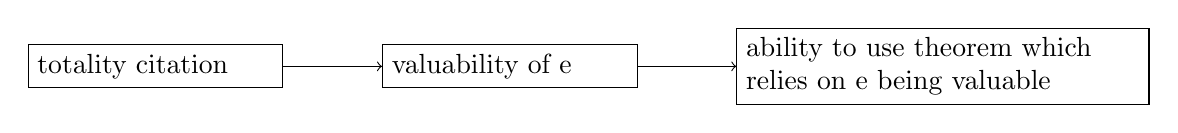
\begin{tikzpicture}
      \node[shape=rectangle,draw=black, text width=3cm] (M1) at (-3,2) {totality citation};
      \node[shape=rectangle,draw=black, text width=3cm] (M2) at (1.5,2) {valuability of \code{e}};
      \node[shape=rectangle,draw=black, text width=5cm] (M3) at (7,2) {ability to use theorem which \\ relies on \code{e} being valuable};

      \draw[->] (M1) -- (M2);
      \draw[->] (M2) -- (M3);
    \end{tikzpicture}
  \end{center}
\end{frame}

\begin{frame}[fragile]
  \frametitle{A List-Tree Equivalence: Recursive Case}

  Back to the proof.

  \pause
  \vspace{\fill}

  RHS:
  \begin{align*}
    & \code{listSum (inord (Node (L, x, R)))} \\
    &\eeq \code{listSum ((inord L) @ (x :: inord R))} 
    & \tag{clause 2 of \code{inord}} \\
    &\eeq \code{listSum (inord L) + listSum (x :: inord R)}
    & \tag{lemma 1, lemma 2} \\
    &\eeq \code{listSum (inord L) + x + listSum (inord R)}
    & \tag{clause 2 of \code{listSum}, lemma 2} \\
    &\eeq \code{treeSum L + x + treeSum R}
    & \tag{inductive hypothesis, twice}
  \end{align*}

  Now we match the left-hand side, so we can conclude the equivalence.

  \pause
  \vspace{\fill}

  So by the principal of structural induction on trees, we have proven
  that for all values \code{T : tree}, 
  \code{treeSum T} $\eeq$ \code{listSum (inord T)}.
\end{frame}

\sectionSlide{4}{Datatypes}

\begin{frame}[fragile]
  \frametitle{Back to Lists}

  Now that we've seen trees, let's return to lists for a bit.

  \pause
  \vspace{\fill}

  We've seen that we can extract the first element of a list easily by
  using pattern matching. It's not as clear what to do, however, to obtain
  the last element in the list!

  \pause
  \vspace{\fill}

  Let's write a recursive \code{last} function to achieve this.

  \pause
  \begin{codeblock}
    fun last ([] : int list) : int = (* ??? *)
  \end{codeblock}

  \pause
  \vspace{\fill}

  We find that we immediately encounter a problem, however.
\end{frame}

\begin{frame}[fragile]
  \frametitle{Slide to the Left}

  Before we even write the recursive case, we have to write the case for
  the empty list.

  \pause
  \vspace{\fill}

  What is the last element in the empty list? We want to return an
  \code{int}, so it could be \code{0}, or \code{1}, or something arbitrary.

  \pause
  \vspace{\fill}

  The bigger issue is that it simply doesn't make sense to return an integer
  for this function. We want to return something else, to distinguish the
  cases of "found 0" and "found nothing".
\end{frame}

\begin{frame}[fragile]
  \frametitle{An Optional Type}

  There are quite often times where we want to write a function, where some inputs
  do not have a well-defined answer.

  \pause
  \vspace{\fill}

  We've seen this with the \code{div} and \code{fact} functions, where \code{0} and 
  negative numbers cause an exception to be raised, and infinite looping, respectively.

  \pause
  \vspace{\fill}

  Sometimes, we don't want such things to happen, however. We would prefer to return
  a value, which is a more predictable and safe behavior.

  \pause
  \vspace{\fill}

  To facilitate this, we have the \code{option} \term{type constructor}. 
\end{frame}

\begin{frame}[fragile]
  \frametitle{Type Constructors}

  A \term{type constructor} is something which makes a type out of other types. 

  \pause
  \vspace{\fill}

  We were brief about this previously, but that is exactly what \code{list} is!
  Out of the types \code{int}, \code{bool}, and \code{int list}, we can make
  the types \code{int list}, \code{bool list}, and \code{int list list}.

  \pause
  \vspace{\fill}

  Similarly, we will be able to construct the types \code{int option}, \code{string option},
  and \code{int list option}.
\end{frame}

\begin{frame}[fragile]
  \frametitle{The \code{option} Type Constructor}

  \tgs

  \defBox{}{\, For any type \code{t}, there is a type \code{t option}, which describes
  a value that is \textit{possibly} a value of type \code{t}}.
  
  \pause
  \vspace{\fill}

  The type \code{t option} has the following constructors:
  \pause
  \begin{itemize}
    \item \code{NONE}, which is a constant constructor of no arguments \pause
    \item \code{SOME : t -> t option}, which is a constructor that takes
    a single argument of type \code{t}.
  \end{itemize}

  \pause
  \vspace{\fill}

  So for instance, here are some examples of options:
  \begin{itemize}
    \item \code{SOME 5 : int option}
    \item \code{SOME [] : int list option}
    \item \code{NONE : int option}
    \item \code{NONE : bool option}
  \end{itemize}
\end{frame}

\begin{frame}[fragile]
  \frametitle{Get Thee To A \code{NONE}-ery}

  Let's rewrite \code{last} with this knowledge!

  \pause
  \vspace{\fill}

  \begin{codeblock}
    fun last ([] : int list) : int option = NONE
      | last [x] = SOME x
      | last (x::xs) = last xs 
  \end{codeblock}

  \pause
  \vspace{\fill}

  We could have raised an exception, but this behavior gives more
  agency to the caller of the function, in case they want to do something
  when the list has no output value.
\end{frame}


\begin{frame}[fragile]
  \frametitle{Datatypes}

  So far, we've seen a few examples of type which have different \term{variants},
  or kinds of constructors that make up the values of the type.

  \pause
  \vspace{\fill}

  Lists, for instance, can be \code{[]} or \code{x::xs}, trees can be \code{Empty}
  or \code{Node(L, x, R)}, and options can be \code{NONE} or \code{SOME x}.

  \pause
  \vspace{\fill}

  These are all known as \term{variant types}, or \term{sum types}, and can be 
  defined using the \code{datatype} keyword! They define all the forms that
  values of a type can take, and \textit{no more}.

  \pause
  \vspace{\fill}
  
  \begin{codeblock}
    datatype int_option = NONE | SOME of int

    datatype int_list = [] | :: of int * int list
  \end{codeblock}
\end{frame}

\begin{frame}[fragile]
  \frametitle{Framing the Problem}

  Defining types that fit the shape of the problem is one of the strongest
  aspects of a functional programming language. These types are known as 
  \term{algebraic datatypes}.

  \pause
  \vspace{\fill}

  For instance, suppose we are interested in an ordering function on integers, 
  which has type \code{int * int -> order}. What should we define the type of
  \code{order} to be?

  \pause
  \vspace{\fill}

  There are three possibilities. The first is less than the second, they are
  equal, or the first is greater than the second. \code{bool} will not suffice
  here!
\end{frame}

\begin{frame}[fragile]
  \frametitle{The \code{order} type}

  We could use the description of their relationship as the output value.
  We can use a \term{type alias} to alias the name \code{order} to be the
  same as the name \code{string}.

  \pause
  \vspace{\fill}

  Then, we define our \code{compare} function:

  \vspace{\fill}

  \begin{codeblock}
    type order = string 

    fun compare (x : int, y : int) : order = 
      if x < y then
        "less"
      else if x = y then
        "equal" 
      else
        "greater" 
  \end{codeblock}
\end{frame}

\begin{frame}[fragile]
  \frametitle{A Fragile Approach}

  This approach is needlessly fragile, however. What does the code look like
  for a consumer of this function?

  \pause
  \vspace{\fill}

  \begin{codeblock}
    case compare (x, y) of
      "LESS" => (* code for the less case *)
    | "EQUAL" => (* code for the equal case *) 
    | "GREATER" => (* code for the greater case *)
    | _ => (* shouldn't be possible??? *)
  \end{codeblock}

  \pause
  \vspace{\fill}

  When casing on the result of \code{compare}, the compiler doesn't know that
  any case other than \code{"LESS"}, \code{"EQUAL"}, and \code{"GREATER"} is
  impossible! This necessitates a redundant extra case.
  
  \pause
  \vspace{\fill}

  What's another issue with the above code?

  \note {
    It's all wrong! I intentionally misspelled the strings, so actually the code
    we wrote would always enter the "impossible" case.
  }
\end{frame}

\begin{frame}[fragile]
  \frametitle{A Fragile Approach}

  The point is that, although it is \textit{possible} to have \code{order} be the
  same as \code{string}, it comes with a great deal of flaws.

  \pause
  \vspace{\fill}

  Programming isn't about the possibility of the solution, it's about finding the
  \textit{best} solution. It's an inherently linguistic process, and we're interested
  in having good grammatical structure.

  \pause
  \vspace{\fill}

  We can use datatype declarations to solve this problem in a better way.
\end{frame}

\begin{frame}[fragile]
  \frametitle{The \code{order} datatype}

  Let's define our own \code{datatype} that fully captures the cases that
  we are interested in.

  \pause
  \vspace{\fill}

  \begin{codeblock}
    datatype order = LESS | EQUAL | GREATER

    fun compare (x : int, y : int) : order = 
      if x < y then
        LESS
      else if x = y then
        EQUAL 
      else
        GREATER 
  \end{codeblock}
\end{frame}

\begin{frame}[fragile]
  \frametitle{Communication, Better}

  \tgs

  Now, downstream consumers of this function can write the following code:

  \pause
  \vspace{\fill}

  \begin{codeblock}
    case compare (x, y) of
      LESS => (* code for the less case *)
    | EQUAL => (* code for the equal case *) 
    | GREATER => (* code for the greater case *)
  \end{codeblock}

  \pause
  \vspace{\fill}

  There's no need to have an extra redundant case, and now the compiler will
  warn if you misspell one of the variants.

  \pause
  \vspace{\fill}

  This leads to much more polished, streamlined code! Remember the mantra,
  \term{Types Guide Structure}. We use the power of types to structure our
  solution to a problem.
\end{frame}

\sectionSlide{5}{Type Casting}

\begin{frame}[fragile]
  \frametitle{A People Problem}

  Problems come in all shapes and sizes. The great strength of algebraic datatypes
  is in being able to craft a type representation that exactly describes your problem.

  \pause
  \vspace{\fill}

  For instance, suppose we have a class of people. Some people are employed, some
  people are students, and some people are unemployed.  

  \pause
  \vspace{\fill}

  We might be interested in a couple of things:
  \begin{itemize}
    \item the person's name
    \item the person's paycheck, if employed, and tuition, if a student
    \item the company an employed person works for 
    \item the amount of courses a student is taking
    \item days since last employed, if unemployed (if ever)
    \item title of last job, if unemployed (if ever)
  \end{itemize}
\end{frame}

\begin{frame}[fragile]
  \frametitle{Class Description}

  In service of this, we might define a following datatype which describes a person:
  \begin{codeblock}
    datatype class = Employed | Student | Unemployed
  \end{codeblock}

  \pause
  and the following type which describes the above information:
  \begin{codeblock}
    type person_info =
      string (* name *)
      * real (* positive paycheck, if employed. negative 
                tuition, if a student, and 0 if unemployed *)
      * string option (* company name, if employed, o.w. NONE *)
      * int option    (* # of courses, if student, o.w. NONE *)
      * int option    (* days since employment, o.w. NONE *)
      * string option (* last job if unemployed, o.w. NONE *)
  \end{codeblock}
\end{frame}

\begin{frame}[fragile]
  \frametitle{Excessive Invariants}

  We would then say that a person was a tuple of a \code{class} and \code{person_info}.

  \pause
  \vspace{\fill}

  This is very clearly disgusting. There are floating invariants everywhere! 

  \pause
  \vspace{\fill}

  We have to make sure that people who are employed don't have a number of
  courses, or a number of days unemployed, or a negative paycheck!  

  \pause
  \vspace{\fill}

  In addition, we might be interested in applying a totally necessary tuition
  increase. Let's write that function:

  \begin{codeblock}
    fun newTuition (_, tuition, _, _, _, _) = tuition * 1.04
  \end{codeblock}

  \pause
  \vspace{\fill}

  Except now, this function could possibly run on someone who is just
  employed or unemployed. Something really bad could happen because this
  function was written too generically, because the types were all wrong!
\end{frame}

\begin{frame}[fragile]
  \frametitle{A Better Class System}

  Can we do better?

  \pause
  \vspace{\fill}

  Let's try isolating the parts of each person that are relevant, into
  the \code{class} type.

  \pause
  \vspace{\fill}

  \begin{codeblock}
    type class =
        Employed of real * string  
          (* paycheck and company name *)
      | Student of real * int 
          (* tuition and # of courses *)
      | Unemployed of (int * string) option
          (* days unemployed and last employer *)

    type person = string * class
  \end{codeblock}
\end{frame}

\begin{frame}[fragile]
  \frametitle{A Better Class System}

  We see that every person has a name, so \code{string} can be factored out. We 
  can isolate things like company name and number of courses to specific cases,
  and eliminate the \code{real} from unemployed people entirely.

  \pause
  \vspace{\fill}

  For unemployed people who have had previous jobs, we notice that days unemployed and
  last employer should only be set if both are set, so we fold them both into a 
  single tuple, and make it an \code{option}, if the person was never employed.
\end{frame}

\begin{frame}[fragile]
  \frametitle{Type Casting}

  \tgs

  This is a phenomenon I call \term{type casting}. This is not anything to do 
  with the typical definition of type-casting, involving free conversion of 
  values of one type to another, which does not exist in SML.

  \pause
  \vspace{\fill}

  \defBox{}{\, Similarly to how a blacksmith casts metals to fit a mold of what
  they need, \term{type casting} is the art of designing types in a way that
  they fit the specification of the problem at hand.}

  \pause
  \vspace{\fill}

  An imperative programmer tries to fit square pegs into round holes. A 
  functional programmer can \textit{make} a peg to fit any hole that they need.
\end{frame}

\begin{frame}[plain]
	\begin{center} Thank you! \end{center}

	\begin{center} 
    Post-lecture survey: \\
    \vspace{5pt}
    \includegraphics[scale=0.035]{qr_may25}
  \end{center}
\end{frame}

\end{document}

